\chapter{Background and related work}
\label{chap:background}
\section{Decoding from (i)EEG signals}
Neural decoding refers to a neuroscience field concerned with the reconstruction of external stimuli from information that is already encoded in the brain.
It consists of multiple stages, namely, signal recording, spectral and spatial feature extraction and the final classification or regression algorithm, depending on the type of the decoding task. 
In this chapter, we describe the methods traditionally used in each of these stages highlighting their advantages and disadvantages. 
While many things, such as sleep stages \cite{sleep-eegnet}, epileptic seizures \cite{epileptic-seizures-eeg} or emotions \cite{} can be decoded from brain signals, we introduce mainly methods used for movement decoding because they are most relevant for this thesis. 

\subsection{Recording methods}
An existing correlation between neural modulations and motor parameters for a wide range of motor tasks makes electrical brain activity suitable for movement decoding  \cite{lebedev-cortical-2005}.
Electroencephalography (EEG), electrocorticography (ECoG) and stereotactic EEG (sEEG) are the most commonly used techniques of recording electrical activity of the brain \cite{tam-human-2019}.
We describe basic properties of each of these methods. For a more detailed introduction to EEG please refer to \cite{NiedermeyersElectroencephalography}.

\subsubsection{Electroencephalography (EEG)}
Electroencephalography (EEG) records electrical brain activity of the cerebral cortex using multiple electrodes (also called channels) which are placed on the surface of the head. The recorded activity, originating as the postsynaptic potential of excitable neural tissue \cite{buzsaki-origin-2012}, is attenuated through cerebrospinal fluid, the dura and the skull on its way to the recording electrodes. Besides weakening the signal, these structures also act as low-pass filters limiting the useful frequency bands to below 100~Hz \cite{tam-human-2019}. Another limitation of EEG recordings is the interference of muscle activity in the region of the head. Muscle activity has a higher amplitude than brain signals and can therefore affect the recording quality \cite{scholg-presence-2002}. Despite a low signal-to-noise ratio and also poor spatial resolution, EEG is a widely used tool in brain signal recording. Its high temporal resolution, safety and a relatively low cost motivate researchers to develop new quality control and artifact processing techniques \cite{} to alleviate the above mentioned disadvantages. 

\subsubsection{Electrocorticography and stereotaxic EEG}
Electrocorticography (ECoG) and streotaxic electroencephalography (sEEG) are variations of EEG commonly referred to as intracranial EEG (iEEG).
In ECoG, a grid with multiple recording electrodes is placed on the surface of the brain instead of the surface of the head.
For stereotaxic EEG, the electrodes penetrate the skull and they reach deeper inside the brain. Both are very invasive methods and cannot be performed for the sake of research only.
Therefore, intracranial EEG studies are mainly conducted on patients with medication resistant epilepsy.
The electrodes are used to find the locus of seizures which then is surgically removed. Special measures have to be taken to remove channels displaying pathological symptoms when using ECoG signal for research.
The quality of signal from non-epileptical brain tissue is, however, superior to standard EEG. It has higher spatial resolution as well as better resolution in the high frequencies.

\subsection{Feature extraction}
End-to-end learning has started to be used only recently and manual feature extraction is still common when designing movement decoders.
We will describe some widely used feature extraction methods. 
Often distinct methods are used for spatial and temporal information both of which are present in EEG and iEEG signals. 
Spatial information tells us where in or on the brain the signal was measured depending on the position of the electrode.
Temporal information contains information about when the signal was recorded and what its value was in that moment.
\subsubsection{Spatial feature extraction}
Spatial feature extraction methods are used for signal denoising, rejection of pathological channels and dimensionality reduction.
 Common average reference (CAR) is a widely used and simple method where from each channel, the mean of all channels is subtracted \cite{liu-effects-2015}. This reduces noise common to all channels but might introduce some channel specific noise to some otherwise clean channels \cite{volkova-review}. Multiple other methods have been proposed to address this issue. For example autoregressive models which instead of subtracting the average of the channels assign a weight to each channel so that it minimizes the variance and then subtract this weighted average from each channel \cite{adaptive-laplacian-reference}. Bipolar reference and Laplacian reference \cite{yao2019reference, laplacian-reference} are also ways to avoid proposing channel specific noise by focusing only on re-referencing of neighbouring channels. \\
 
Noisy and epileptic channel rejection is often done after visual inspection by experts. Nevertheless, automatic mechanisms to select channels for removal have also been developed. A noisy channel can be identified based on an abnormal distribution, identification of excessive line noise or outliers it contains. If a channel is marked noisy, it is removed from the dataset. However, some studies propose the use of CAR with median subtraction instead of mean and keeping all channels. They claim that this way we retain all information possibly valuable for decoding while also sufficiently reducing noise across all channels \cite{liu-effects-2015}. \\

Recording from multiple electrodes creates highly dimensional data. Reducing their complexity is another opportunity for spatial feature extraction to help achieve better decoding results. Principal component analysis (PCA) is a commonly used method \cite{}. It transforms the data into a new coordinate system achieving largest possible variance along the axes. Optionally, one can then discard the axes with the lower variance. Independent component analysis, another tool for dimensionality reduction similarly transforms the data into a new coordinate system. Unlike PCA, it selects a basis in which each vector is an independent component of the data \cite{ica}

\subsubsection{Spectral feature extraction}
Spectral feature extraction methods are used to extract task-related features from the time-domain and power spectra domain. Regarding the time-domain, the Low-pass filtered component (LFC), also called Local motor potential (LMP) which can be extracted using Savitzky-Golay filters \cite{multitaper-31} has been shown by multiple studies to hold information about movement time-course and kinematics \cite{schalk-2007, Pistohl2008PredictionOA, ball-2019}. In the power spectrum domain, following are the traditionally defined frequency ranges:$\delta$ (0–4~Hz), $\theta$ (4–8~Hz), $\alpha$ (8–12~Hz), $\beta$ (13–30~Hz), low $\gamma$ (30–50~Hz) and in the case of ECoG high $\gamma$ band (50~Hz and above) \cite{hammer-predominance-2016}. The modulations in the alpha, beta and in the case of intracranial EEG also high-gamma bands are particularly informative for movement decoding \cite{ball-hg-importance, 34-gunduz-hg}. The signals in the alpha and beta bands are not tied to a specific location, whereas the high-gamma reflects the local activity of spiking neurons. As previously stated, the high-gamma signal from EEG is often noisy and not suitable for decoding. However, it has been shown that neural networks are able to use information from the high-gamma band for movement classification \cite{schirrmeister-deep-2017}.  \\

 Multiple methods have been proposed to extract features from the power spectrum domain. 
 The signal can be either directly band-filtered in the desired range or converted into the frequency domain using both non-parametric or parametric methods. 
 Non-parametric methods include Fourier analysis, multi-taper methods and wavelet transformations \cite{36-vugt-2007}. 
 Fourier analysis involves convolving the brain signal with a sinusoidal function of a fixed length. The analysis is performed on short windows to improve temporal specificity, nevertheless, its time-frequency resolution is quite poor.
 Moreover, it is only useful in a limited frequency range, based on the window size and the size fixes also the scale of the signal that is to be detected. 
Both multi-tapering methods and wavelets were designed to ameliorate these issues. 
Decomposing the signals into shifted and scaled versions of an oscillating waveform of a wavelet function allows the proportion between the temporal width and frequency band-with to stay the same for all frequencies. 
This contributes to a higher temporal resolution in higher frequencies. The good time-frequency trade-off of wavelets makes them suitable for analysing non-stationary signals.  \\

Multi-taper methods were designed to reduce bleeding between frequencies making them also well-suited for analyzing signals of non-stationary processes. 
Tapers are functions having a value of one in the middle and then taper to zero at the edges. 
The multi in multi-taper implies that the signal is convolved with multiple orthogonal tapers.
These are then averaged yielding a statistically consistent spectral estimator with reduced variance of the spectral estimates and improved localisation in the frequency domain \cite{multitaper-31}. 
Auto-regressive spectral estimators (AR) are parametric spectral feature extractors. They have proven successful for modelling both EEG \cite{auto-regressive-eeg} and iEEG \cite{anderson-offline-2009}. 
Even though ARs have an inherent capacity to model peaky spectra characteristic for bio-signal, their effectivity largely depends on parameterization, which is not particularly straight-forward \cite{anderson-offline-2009}. \\

More recently proposed approaches based on Riemann geometry which use covariance matrices to for feature learning and representation have shown promising results \cite{}. 
Temporal modulations can also be modeled problematically using hidden Markov's models or conditional random fields \cite{markov-models-decoding, bayesian-decoding}. 
Importantly also neural networks can also be integrated in the movement decoding pipe-line as of feature extractors. For example auto-encoders are suited for dimensionality reduction.
An auto-encoder consists of two parts.
The encoder first compresses the data into a smaller representation.
The decoder then receives the compressed data and without information about their initial form tries to reconstruct them. This forces the encoder to create a smaller representation which, however, contains as much information as possible. 
Convolutional neural networks are also particularly useful in signal processing because many of the aforementioned filters can be implemented as convolutions. \\



\subsection{Classification methods}
Various movement related classification tasks such as wrist flexion or extension \cite{}, grasp type classification \cite{}, movement of individual fingers \cite{cond-rf-finger-class, lda-finger-movement-classification} or feet movement \cite{} from EEG and iEEG have been studied using a diverse population of classifiers.  
The classifiers include Support vector machines (SVM) \cite{svm-alg}, Linear Discriminant analysis (LDA) \cite{lda-paper}, Quadratic discriminant analysis (QDA) \cite{qda-paper} and their adaptive versions which have gained popularity in the last ten years \cite{lotte2018review} and probabilistic methods such as conditional random fields or naive bayes classifiers \cite{}. \\


\subsection{Regression methods}
Regression tasks are solved less often than classification tasks \cite{volkova-review}.
Movement decoding tasks which fall in the category of regression include finger position decoding \cite{Pistohl2008PredictionOA}, hand position decoding \cite{ball-2019} or
kinematic variables such as speed or velocity decoding of hand movements \cite{hammer-role-2013, hammer-predominance-2016, Hammer-2021, kalman-filters-velocity, linear-regression-eeg-hand-3d}.
Various algorithms have been employed to solve the above listed tasks. 
Models based on linear regression combined with various feature extraction methods are very common \cite{hammer-role-2013, hammer-predominance-2016, eeg-hand-moving, linear-regression-eeg-hand-3d}.
More sophisticated models include Kalman filters \cite{kalman-filters-velocity} or their unscented versions \cite{uns-kalman-filters-gait-decoding}.
Neural networks which we describe separately in Section \ref{sec:dnn-decoding} have also been proposed to solve movement related regression tasks.


\section{Artificial neural networks}
In this section we provide a quick overview of the fundamentals of deep learning (DL) with artificial neural networks. We introduce basic prinicples relevant for this thesis and the related terminology.

\subsection{Convolutional neural networks}
Deep neural networks (DDNs) are statistical machine learning models which are somewhat based on the functioning of the brain.
The networks are composed of interconnected neurons also called units.
A neuron is defined as a weighted sum of its inputs followed by a activation function which is usually non-linear.
In deep neural network architectures, multiple interconnected layers of neurons are stacked on top each other, thus the depth in the term.
The neurons in the layers can be interconnected in various ways.
Feed-forward networks are such that the connections do not form a cycle.
The outputs of the preceding layer are always used as inputs of the following one. 
Networks in which their connections do form cycles are called Reccurent neural networks (RNNs). 
For more information on RNNs please refer to \cite{reccurent-neural-networks}. \\

Considering feed forward networks a simple approach of connecting neurons between two layers is connecting every pair of neurons. 
Consider layers $A$ with a neurons and $B$ with b neurons.
The output of a neuron k from layer $B$ is then defined as:
\begin{equation}
    y_k=f(\sum_{i=1}^{a}x_i*w_{i,k})
\end{equation}

where $f$ is the activation function, $x_i$ is the output of neuron $a_i$ and $w_{i, k}$ is the weight between neuron $a_i$ and $b_k$. An example of a simple three-layer fully connected neural network is displayed in Figure \ref{fig:simple-net}
\begin{figure}[!htpb]
\centering
   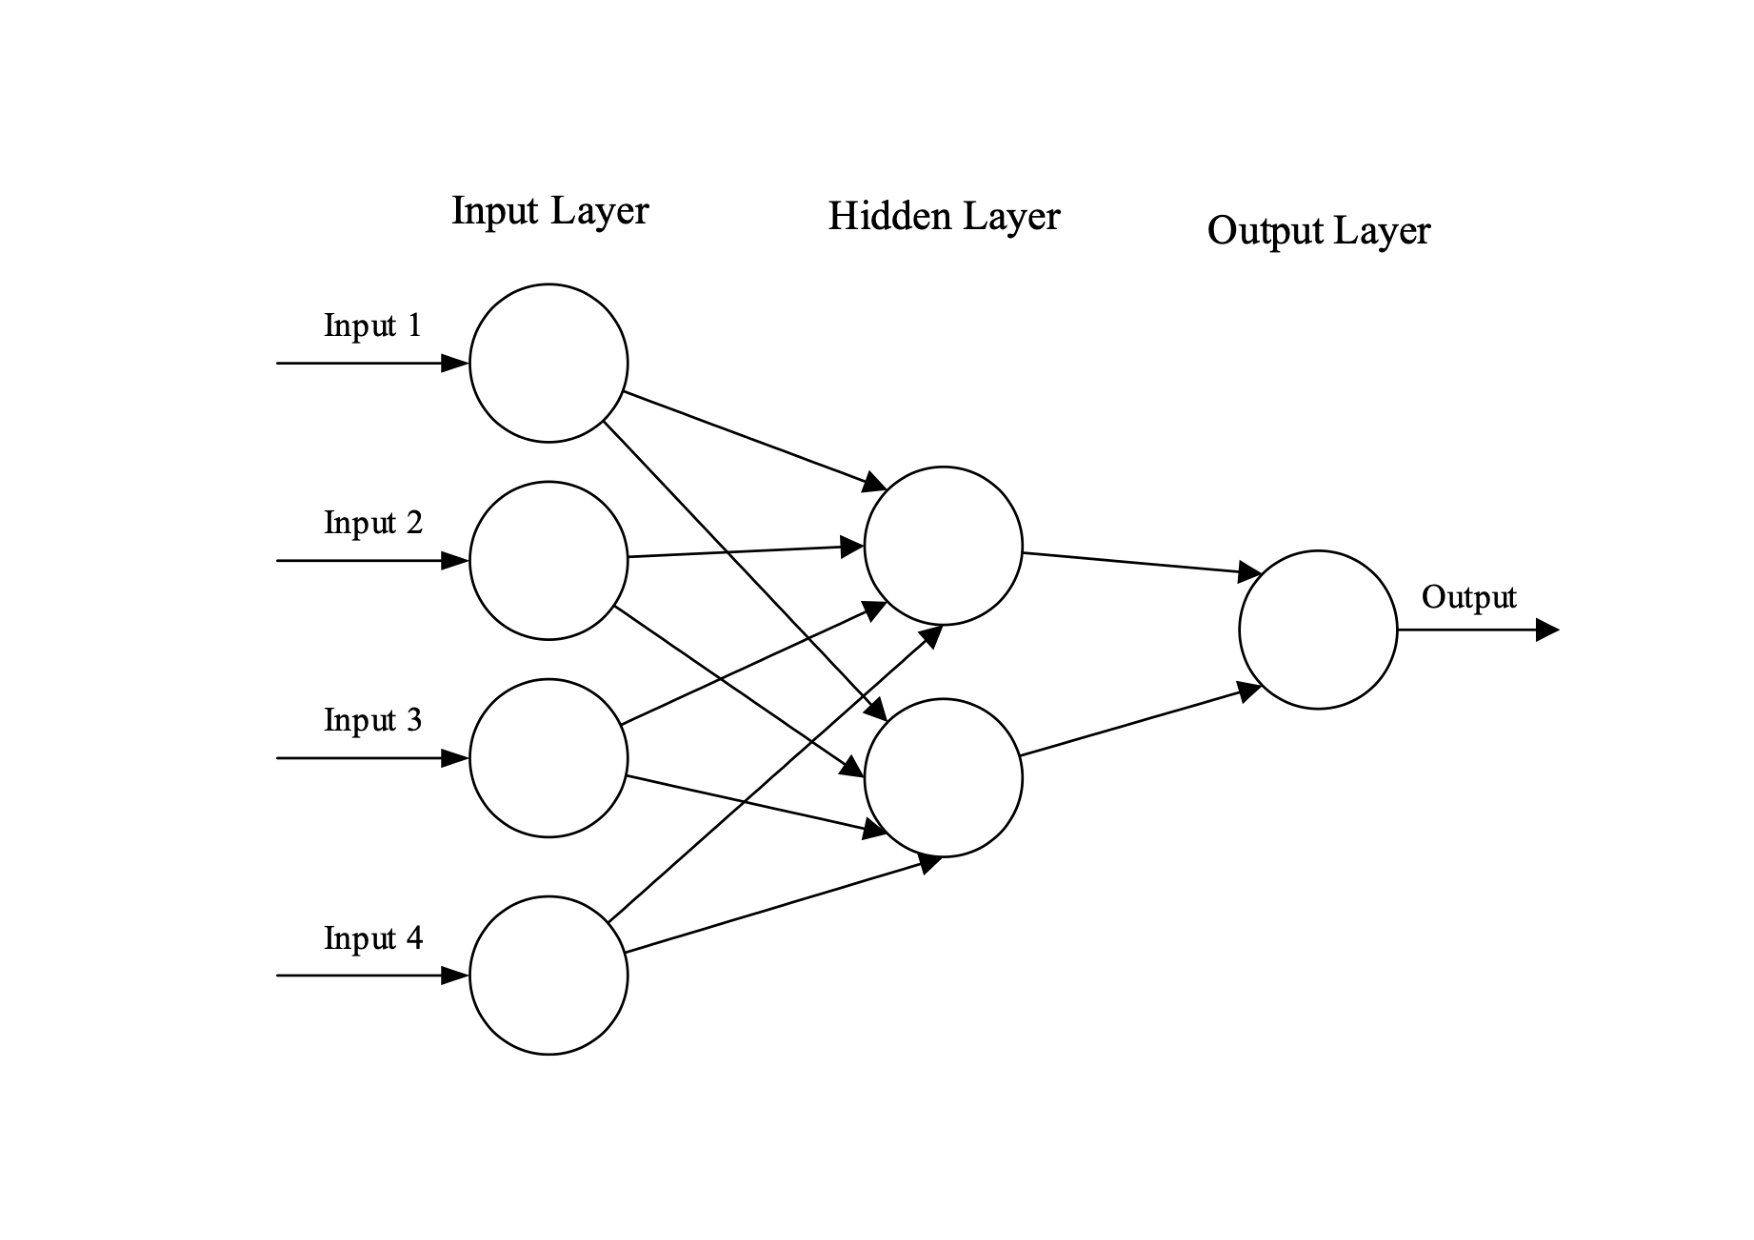
\includegraphics[width=0.8\linewidth]{img/ch2/simple-net}
   \caption[Convolutional filter]{An example of a three-layer fully connected feed-forward network taken from \cite{conv-intro}}.
\end{figure}\label{fig:simple-net}

Besides assigning a separate weight for each pair of neurons there is another possibility.
We can create a smaller weight matrix, often called filter or kernel which be used to perform convolution (i. e. a sliding dot product between the filter and a correspondingly sized part of the layer's input matrix). 
For visual explanation see Figure \ref{fig:convolution}.
To arrive at a complete convolutional layer from the convolutional filter, more parameters need to be specified:
\begin{itemize}
    \item $W$  and $H$ - the width and height of the kernel
    \item $D$ the depth of the kernel. 
    It specifies how many input channels the layer's input has.
    What channels can represent can be illustrated for example on images.
    Imagine a colored image of size 32x32 pixels.
    Besides the width and height the image also has a 3rd dimesion - 3 channels specifying the RGB color.
    Therefore, the dimension of the input (the image) is 32x32x3 and the kernel sliding over it has to have an additional dimension to handle the three input channels - the depth.
    \item $F$ - the number of output channels. 
    It specifies the number of different filters of size $WxHxD$ which all slide over the input giving $F$ output channels. 
    Similarly to the RGB channels of the input described above, each of the different filters allows the network to create its own representation of some feature of the layer's input.    
    \item \textit{stride} - it specifies by how many input points the kernel is shifted when sliding over the input. 
    \item \textit{padding} - specifies if only valid inputs should be taken into account or if the input is to be padded when the kernel reaches outside of the original input.
    If no padding is involved, the size of the output decreases along the dimension where kernel size of the filter is not 1.
\end{itemize}

Considering a 2D convolutional layer having input $I$ with $D$ input channels and parametrized by a kernel $K$ of total size $WxHxDxF$ the output of the layer before the activation function is computed as:

\begin{equation}
    (K \convolution I)_{i,j,o} = \sum_{m,n,d} I_{i*s_1+m,j*s_2+n,c} K_{m,n,c,o}
\end{equation}\label{eq:convolution}

where $s_1$ and $s_2$ are strides in the corresponding dimensions, c are the input channels and o are the output channels.

\begin{figure}[!htpb]
\centering
   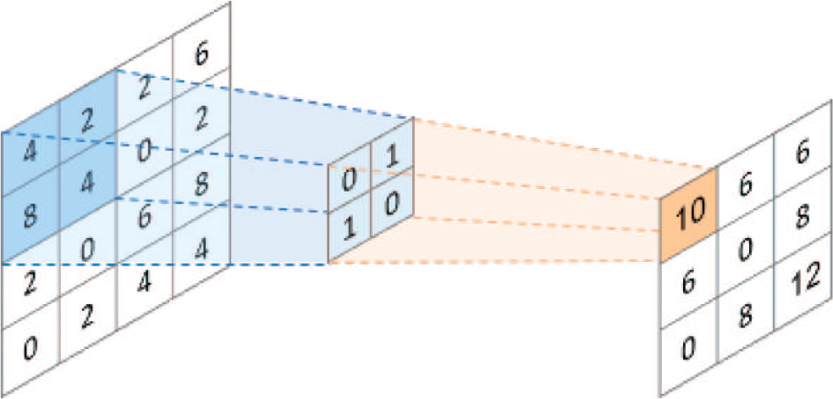
\includegraphics[width=0.8\linewidth]{img/ch2/convolution.jpg}
   \caption[Convolutional filter]{An example of a convolutional filter of width 2 and height 2 with weights 0, 1, 1, 0 sliding over an input of size 4x4 taken from \cite{conv-diagram}}.
\end{figure}\label{fig:convolution}

When a network contains one or multiple layer performing convolution, such a network is called a convolutional neural network (CNN).
Convolutional layers are often supplemented with pooling layers such as max-pooling or average pooling which aim to achieve shift-invariance in CNN architectures \cite{cnn-description}. 
Common activation functions used in CNNs are sigmoid, tanh, or ReLU \cite{relu-paper}.
More recently also the eLU function which we are using in this thesis \cite{clevert-elu-2016}. \\

\subsubsection{Training}
Deep neural networks tend to have large numbers of parameters and therefore, cannot be trained analytically. Instead, they are trained based on gradient descent based methods such as stochastic gradient descent (SGD) \cite{} or more recently a popular method called ADAM \cite{kingma-adam-2017}. 
To give the reader an idea of the fitting process, we describe it in a simplified manner below. 
First a small subset of the input (a \textit{batch}) is randomly sampled from the training set. 
The batch is used as input into the network and through a forward pass we get the output of the network. 
The output and the \textit{gold labels} (desired output based on the selected inputs) are given to the \textit{loss function} which serves as a indicator of how far the model is from the correct output. 
Finally, the first derivatives of the loss function (the \textit{gradient}) with respect to the parameters of the model are subtracted from these parameters (the \textit{weights}).
This last step in theory decreases the value of the loss function in the next forward pass.
The forward pass is repeated for all batches in the dataset. When all batches pass through the network, we can say one \textit{epoch} was completed. 

\subsubsection{Regularization}
Overfitting - the adaptation to the training set distribution to an extend that the model does not generalize well over unseen data, is an unneglectable problem in deep neural networks including CNNs.
Multiple methods which effectively reduce this this problem have been proposed.
One option is to add a penalization term into the loss function which penalizes the model complexity.
An example of such a regularization is $l_p$-norm regularization \cite{cnn-description}.
Dropout layers \cite{drop-out} also serve as regularization tools. 
By completely dropping some of the connections between neurons randomly, they prevent the network from becoming dependant on single neurons and force it to be able to make good predictions even when some information is absent.
Another popular regularization technique for CNNs is batch normalization \cite{batch-norm} which besides regularization also reduces the internal covariance shift. 
In CNNs this method now often substitutes dropout layers which are more suited for fully connected layers \cite{cnn-description}.


\subsubsection{Dilated networks}
Convolutional neural networks are widely used in computer vision, more specifically in pattern recognition where they substantialy raised state-of-the-art \cite{alexnet, dnn-computer-vision} and their localized focus is well suited to image processing.
Nevertheless, CNNs are increasingly used for dense predictions.
Dense prediction in the sense of computer vision means assigning one label to each pixel of an image \cite{dense-prediction-images}. 
But this notion of one output per one input point can be extended to other fields such as machine translation \cite{dense-prediction-machine-translation}, speech synthesis \cite{wavenet} or prediction from EEG \cite{schirrmeister-deep-2017} and iEEG \cite{Hammer-2021}.
The above metioned tasks were solved using CNNs when a new parameter called dilation was introduced \cite{dense-prediction-images}.
Dilation inserts zeros between the elements of the convolutional filter and so enlarges the CNNs receptive field allowing it to cover more relevant information.
For a visual explanation of dilation see Figure \ref{fig:dilation}.

\begin{figure}[!htpb]
\centering
   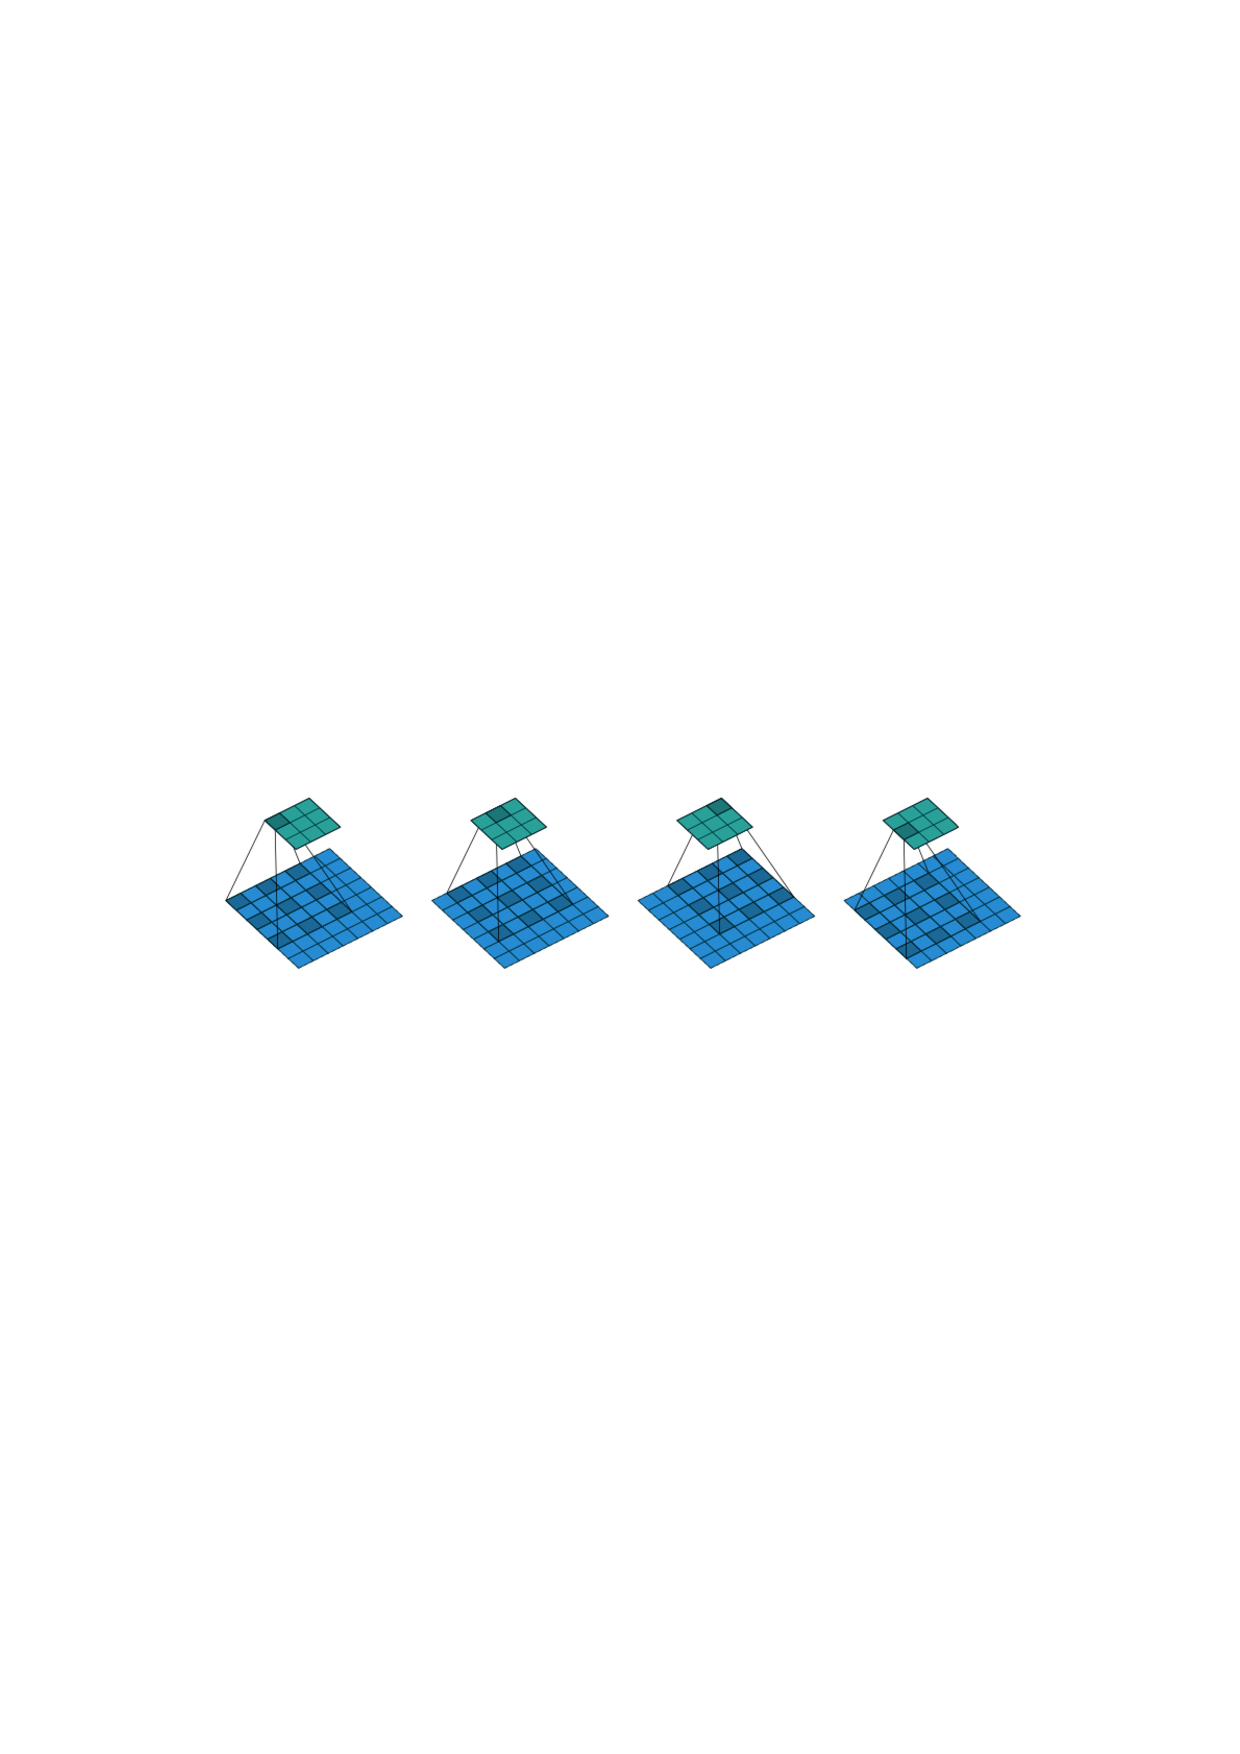
\includegraphics[width=0.8\linewidth]{img/ch3/dilated-conv.pdf}
   \caption[Dilated convolution]{An illustration of a dilated convolution with kernel size (3, 3) and dilation (2, 2) from \cite{dilated-conv}.}
\end{figure}\label{fig:dilation}


\subsection{CNN interpretability}
Poor interpretability of deep neural networks including CNN models has been identified as a major challenge limiting their usefulness across fields. 
Especially in safety-critical fields such as autonomous driving, or medical decision support, it is crucial for us to understand how DNNs arrive at their decisions.
In the case of EEG and iEEG decoding, understanding how networks which are able to translate these signals into for example velocity or speed arrive at their decision would lead to a better understanding of the brains functionality. 
It could also help identify ways in which these networks can be optimized to yield better predictions.
Because the strength of DNNs often lies in large datasets, in a field where data is less available, such optimizations are particularly important.\\

Substantial effort has been made to explain how deep neural networks make their predictions.
Many of the popular methods, such as maximal activating inputs \cite{maximizing-activation}, class-activation maps \cite{class-activation-maps}, saliency maps \cite{gradient-visualization} or layer-wise relevance propagation \cite{sturm-interpretable-2016} have been used also in interpreting DNNs used for brain signal decoding \cite{goodfellow-towards-2018, hartmann-hierarchical-2018, rieke-visualizing-2018, yang-visual-2018,  sturm-interpretable-2016, }.

\section{DNNs for (i)EEG decoding}
\label{sec:dnn-decoding}
In this section, we introduce the Deep4Net created by \cite{schirrmeister-deep-2017} which is the main focus of the presented experiments.
Then we go on to describe another paper \cite{Hammer-2021} who used the Deep4Net to do the same task as we are on the same data and laid the foundation of the here presented research.

\subsection{Schirrmeister et al.}\label{subsec:schirrmeister-et-al}
The paper \cite{schirrmeister-deep-2017} published in 2017 by Schirrmeister et al. introduced multiple CNN and hybrid architectures suitable for movement decoding from raw EEG signals, including the Deep4Net.
It has several important contributions.
First of all, it shows that CNNs are able to achieve at least as good performance on classification from raw EEG signals as the widely used Filter bank common spatial patterns (FBCSP) do from manually extracted features. Besides that, it shows that recent advances in machine learning such as batch normalization or the exponential linear unit (ELU) transfer function help boost the decoding accuracy of the networks on the movement decoding task.
Lastly, using a perturbation visualization method they explore, which spectral power features are important for the network's predictions.
They show there is substantial effect of the frequencies in the alpha and beta band on the networks prediction.
They also observe an effect of the high-gamma freuquencies on the predictions which, they claim, is for the first time when using non-invasive EEG data.\\

\subsubsection{Classification task}
Two datasets were used to estimate the abilities of the introduced architectures.
One was the BCI IV 2a competition dataset \cite{brunner2008bci} where the task was to classify motor imagery tasks of 9 subjects imagining to move the right hand, left hand, both feet or tongue.
The second dataset they used was one they acquired in their lab called High Gamma dataset (HGD) as it is especially well-suited for extracting information from high frequencies.
Two additional datasets were used to estimate if the main results hold also on other datasets. 
To this extend the BCI IV 2b competition and the Mixed Imagedy Dataset (MID) were used and confirmed their findings.


\subsection{Hammer et al.}\label{subsec:hammer-et-al}
In 2021, Hammer et al. \cite{Hammer-2021} used the Deep4Net architecture for regression on intracranial EEG.
Differing from the original Deep4Net paper \cite{schirrmeister-deep-2017}, not only in the type of task but also in the kind of data, they inspected the performance of the architecture in these altered settings.
They also visualized the important spectral features investigating learnt specialization of single network units to either phase or amplitude.
This thesis directly follows up on their research.

\subsubsection{Regression task and performance}
In this paper, Deep4Net was used to predict kinematic variables, namely velocity and absolute velocity (speed) based on intracranial EEG (iEEG) of subjects undergoing pre-surgical epilepsy screening. The subjects were asked to play a simple video game. 
Their task was to use a joystick to control a car driving on a winding track. 
The joystick allowed for left and right movement and the velocity and speed of this movement were recorded along with concomitant iEEG signals. 
The dataset and the task are introduced in more detail in Section \ref{subsec:ieeg-data-preprocessing}.\\

Unsurprisingly, the Deep4Net significantly outperformed linear regression used as a baseline on this task \cite{Hammer-2021}, especially for absolute velocity.
It was not evaluated on a public dataset, therefore, a comparison to more decoding methods is not possible, nevertheless, the correlation values it achieved are quite high \ref{fig:hammer-performance}.  

\begin{figure}[!htpb]
\centering
   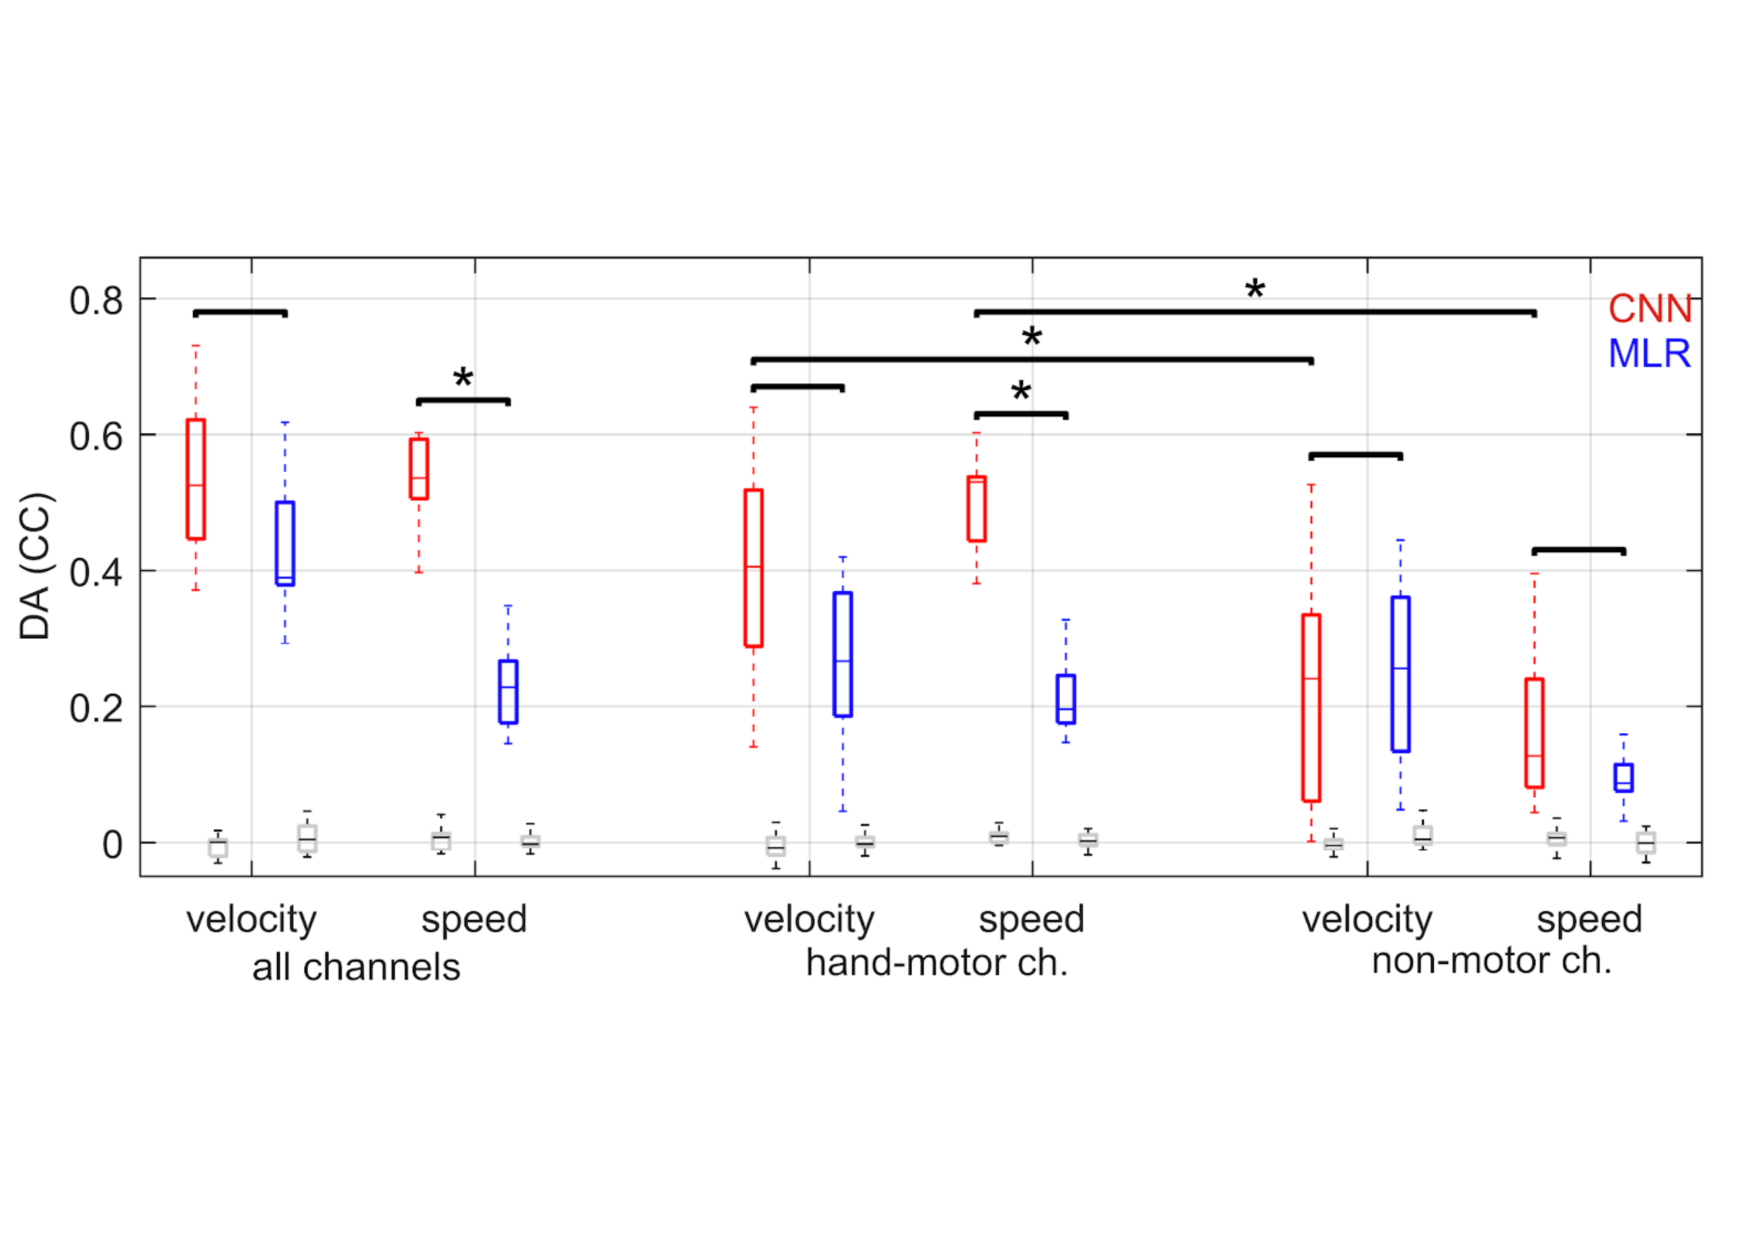
\includegraphics[width=0.8\linewidth]{img/ch2/hammer-decoding-acc.pdf}
   \caption[Orignial Deep4Net performance]{The decoding models for both the Deep4Net (CNN) and multi-linear regression (MLR) used iEEG data from all channels, hand-motor channels, or non-motor channels (see section \ref{subsec:separation-of-motor-and-non-motor-channels}. The performance was assessed by correlation coefficients (CCs) between predicted and real kinematic parameters. In each box-plot, the box indicates the interquartile range (IQR) of the DA distribution across participants, the median is marked by a horizontal line inside the box, the whiskers indicate 1.5-times the IQR. The chance-level CCs for shuffled datasets was assessed for both CNN and MLR (grey box-plots below)\cite{Hammer-2021}}
\end{figure}\label{fig:hammer-performance}

\subsubsection{Training regime}
The Deep4Net was trained using the ADAM optimizer \cite{kingma-adam-2017} with learning rate 0.01 for 100 epochs.
To calculate the error of the networks predictions, the mean squared error (MSE) was used as the loss function.
A leave-one-out-cross-validation on 25 second long data segments (see \ref{subsec:ieeg-data-preprocessing} was employed to estimate the networks performance.
The goodness of prediction was evaluated on the one fold not included in training using the linear Pearson's correlation coefficient \cite{pearson-vii-1895}.
Chance level performance was assessed by randomly pairing the inputs and gold labels. For example iEEG data from fold 2 were paired with gold kinematic data from fold 6.

\subsubsection{Input perturbation - output correlation visualization}
The perturbation analysis in Hammer et al. was more thorough than in the case of \cite{schirrmeister-deep-2017} 
Besides looking at the influence of amplitude perturbations, they also investigated the influence of phase perturbations, similarly to \cite{hartmann-hierarchical-2018}.
Moreover, attention was paid to the specialisation of single units to either phase or amplitude.
While most findings were in line with previous literature, the low sensitivity of the network to the high-gamma frequency bands amplitude was unexpected.  
Especially considering two things: 
1. This same architecture was able to use high-gamma information in EEG decoding where high frequencies contain more noise than in iEEG signal.
2. High-gamma has been shown to be informative in for absolute velocity decoding on a subset of the same data when using linear regression \cite{hammer-predominance-2016}.
Without including it in the research paper, using a different visualization method, namely gradient visualization, they discovered a gradient peak at 83.33~Hz (in the high-gamma band).
The significance of this peak was unclear as it occurred only when the input window to the networks was shortened so that it only had one output (see \ref{subsec:gradinet-visualization}.


\subsection{Related work}
In this section we describe more works which are relevant for movement decoding from EEG or iEEG using deep learning, but are not directly used or referenced in our experiments.
We specifically introduce a few other neural network architectures which have been employed to decode movement related variables. \\


One such networks is the EEGNet \cite{eeg-net}. The authors build a CNN architecture which is able to generalize over different BCI paradigms.
They show that the EEGNet is able to learn a wide variety of interpretable features over a range of different EEG decoding tasks including movement related cortical potentials and sensoroy motor rythms.
An architecture idea recently repeatedly used for decoding from EEG and iEEG signals is combining recurrent layers and convolutional layers to form a hybrid networks. 
Examples of utilizing such networks in movement-related paradigms are \cite{xie-cnn-lstm-finger-movement, Zhang-2019}.
In \cite{xie-cnn-lstm-finger-movement} a network constituting of 4 convolutional layers followed by one LSTM \cite{lstm-paper} layer was utilized to decode individual finger flexion.
In \cite{Zhang-2019}, three convolutional layers followed by three LSMT layers were utilized to solve the BCI IV 2a competition task (same as in \cite{schirrmeister-deep-2017}). 


